\section{Prioritising Brainstorm Ideas}\todo{This section and all that remains of this chapter might be in need of being re-written once the object-oriented methods are inserted.}

Due to the inherent limitations of the project, some functionality has to be excluded. To help determine what functionality should be the focus points, an evaluation is made using the Risk Vs Value model to help prioritising.

The Risk Vs Value model works by having the individual members of the development team evaluate each different functionality individually and giving them a risk and a value. Each of the values and risks is represented by a number between 0 and 100, where 100 means that the functionality on its own will complete the project, and 0 provides nothing to the project. A 100 risk is something that will take all our time, and 0 is done without sacrificing any valuable time. 

In this project, all of the project members individually evaluated, importantly without talking to each other or knowing the evaluation of the other members beforehand. Afterwards, the team compared their results and the participants that differ the most from one another, would each explain why they evaluated it the way they did. After the explanation, the members of the group has the opportunity to change their evaluation. By using this approach, it constructed graph \ref{fig:RiskValueGraph}.

\begin{figure}[!h]
    \centering
	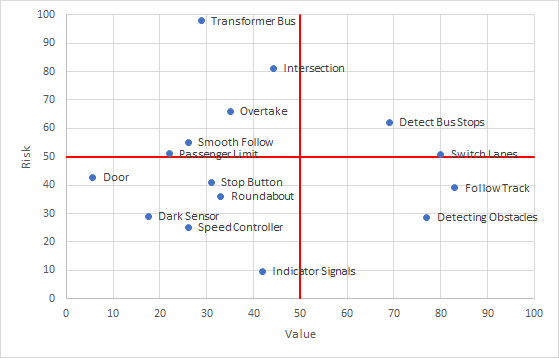
\includegraphics[width=0.9\textwidth]{Images/Graphs/RiskValue.png}
    \caption{Risk Value Graph}
    \label{fig:RiskValueGraph}
\end{figure}

According to the Risk Vs Value model, the development should start with the tasks with a high risk and value, proceeded by the tasks with low risk and high value, and lastly the tasks with a low value and low risk. Where the tasks with high risk and low value were of low priority, or completely ignored. 

According to the graph, detecting bus stops is of first priority, where after further functionality will be prioritised by iterating through the graph clockwise. Noteworthy is that the model is not bulletproof, and as such the relations and dependencies between the different functionality must be taken into account independent of the model.

\subsection{Priority Modifications} % Is this repetition of previous section?

In this section, we will give lower or higher priorities to some features, depending on the relations between the different features.

All of the passenger functionality relies on the driving functionality. Because of this, everything concerning passengers has been deemed of low priority. The same reasoning is given to roundabouts, overtakes and intersections because these also rely on the driving component. Detecting the darkness for turning on lights is also given a low priority based on its low value.

Following the track is crucial, and thus has been given the highest value, and as such has the highest priority.
